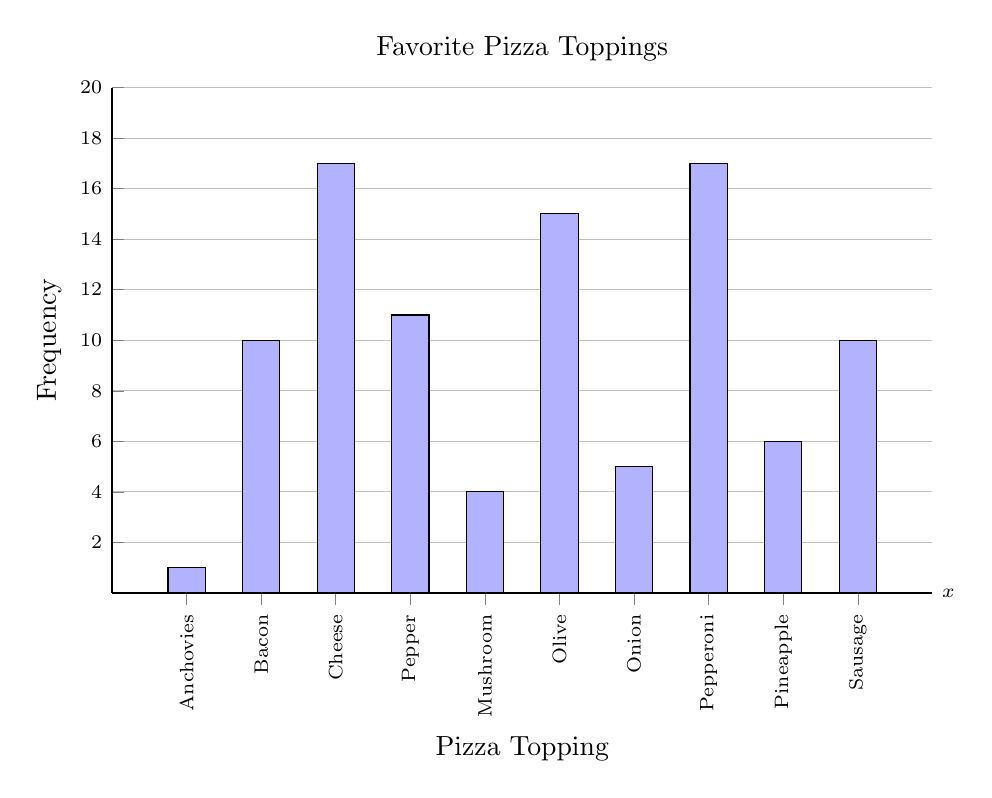
\begin{tikzpicture}[
    declare function={binom(\k,\n,\p)=\n!/(\k!*(\n-\k)!)*\p^\k*(1-\p)^(\n-\k);}
  ]
  \begin{axis}[
      axis lines*=left,
      no markers,
      xmin = 0, xmax=22, ymin=0, ymax=20,
      samples at={2,4,...,20},
      xtick={2,4,...,20},
      ytick={2,4,...,20}, 
      xticklabels={Anchovies,Bacon,Cheese,Pepper,Mushroom,Olive,Onion,Pepperoni,Pineapple,Sausage},
      ticklabel style={font=\scriptsize},
      xticklabel style={rotate=90},
      xlabel={Pizza Topping},
      ylabel={Frequency},
      title={Favorite Pizza Toppings},
      enlargelimits=false,
      clip=false,
      grid = none,
      ymajorgrids=true,
      ybar=0pt, 
      bar width=1,
      width=12cm,
      height=8cm
    ]
    \addplot[fill=blue!30] coordinates { 
        (2,1)
        (4,10)
        (6,17)
        (8,11)
        (10,4)
        (12,15)
        (14,5)
        (16,17)
        (18,6)
        (20,10) };
    \node[right] at (axis description cs: 1,0) {\scriptsize $x$};
  \end{axis}
\end{tikzpicture}
